\documentclass[12pt, notitlepage, final]{article} 

\newcommand{\name}{Vince Coghlan}

\usepackage{amsfonts}
\usepackage{amssymb}
\usepackage{amsmath}
\usepackage{latexsym}
\usepackage{enumerate}
\usepackage{amsthm}
\usepackage{nccmath}
\usepackage{setspace}
\usepackage[pdftex]{graphicx}
\usepackage{epstopdf}
\usepackage[siunitx]{circuitikz}
\usepackage{tikz}
\usepackage{float}
\usepackage{cancel} 
\usepackage{setspace}
\usepackage{overpic}
\usepackage{mathtools}
\usepackage{listings}
\usepackage{color}

\numberwithin{equation}{section}
\DeclareRobustCommand{\beginProtected}[1]{\begin{#1}}
\DeclareRobustCommand{\endProtected}[1]{\end{#1}}
\newcommand{\dbr}[1]{d_{\mbox{#1BR}}}
\newtheorem{lemma}{Lemma}
\newtheorem*{corollary}{Corollary}
\newtheorem{theorem}{Theorem}
\newtheorem{proposition}{Proposition}
\theoremstyle{definition}
\newtheorem{define}{Definition}
\newcommand{\column}[2]{
\left( \begin{array}{ccc}
#1 \\
#2
\end{array} \right)}

\newdimen\digitwidth
\settowidth\digitwidth{0}
\def~{\hspace{\digitwidth}}

\setlength{\parskip}{1pc}
\setlength{\parindent}{0pt}
\setlength{\topmargin}{-3pc}
\setlength{\textheight}{9.0in}
\setlength{\oddsidemargin}{0pc}
\setlength{\evensidemargin}{0pc}
\setlength{\textwidth}{6.5in}
\newcommand{\answer}[1]{\newpage\noindent\framebox{\vbox{{\bf ECEN 3400 Spring 2014} 
\hfill {\bf \name} \vspace{-1cm}
\begin{center}{Homework \#3}\end{center} } }\bigskip }

%absolute value code
\DeclarePairedDelimiter\abs{\lvert}{\rvert}%
\DeclarePairedDelimiter\norm{\lVert}{\rVert}
\makeatletter
\let\oldabs\abs
\def\abs{\@ifstar{\oldabs}{\oldabs*}}
%
\let\oldnorm\norm
\def\norm{\@ifstar{\oldnorm}{\oldnorm*}}
\makeatother

\def\dbar{{\mathchar'26\mkern-12mu d}}
\def \Frac{\displaystyle\frac}
\def \Sum{\displaystyle\sum}
\def \Int{\displaystyle\int}
\def \Prod{\displaystyle\prod}
\def \P[x]{\Frac{\partial}{\partial x}}
\def \D[x]{\Frac{d}{dx}}
\newcommand{\PD}[2]{\frac{\partial#1}{\partial#2}}
\newcommand{\PF}[1]{\frac{\partial}{\partial#1}}
\newcommand{\DD}[2]{\frac{d#1}{d#2}}
\newcommand{\DF}[1]{\frac{d}{d#1}}
\newcommand{\fix}[2]{\left(#1\right)_#2}
\newcommand{\ket}[1]{|#1\rangle}
\newcommand{\bra}[1]{\langle#1|}
\newcommand{\braket}[2]{\langle #1 | #2 \rangle}
\newcommand{\bopk}[3]{\langle #1 | #2 | #3 \rangle}
\newcommand{\Choose}[2]{\displaystyle {#1 \choose #2}}
\newcommand{\proj}[1]{\ket{#1}\bra{#1}}
\def\del{\vec{\nabla}}
\newcommand{\avg}[1]{\langle#1\rangle}
\newcommand{\piecewise}[4]{\left\{\beginProtected{array}{rl}#1&:#2\\#3&:#4\endProtected{array}\right.}
\newcommand{\systeme}[2]{\left\{\beginProtected{array}{rl}#1\\#2\endProtected{array}\right.}
\def \KE{K\!E}
\def\Godel{G$\ddot{\mbox{o}}$del}

\onehalfspacing

\begin{document}

\answer{}
1) \textbf{14.9:}
\begin{figure}[H]
\begin{center}
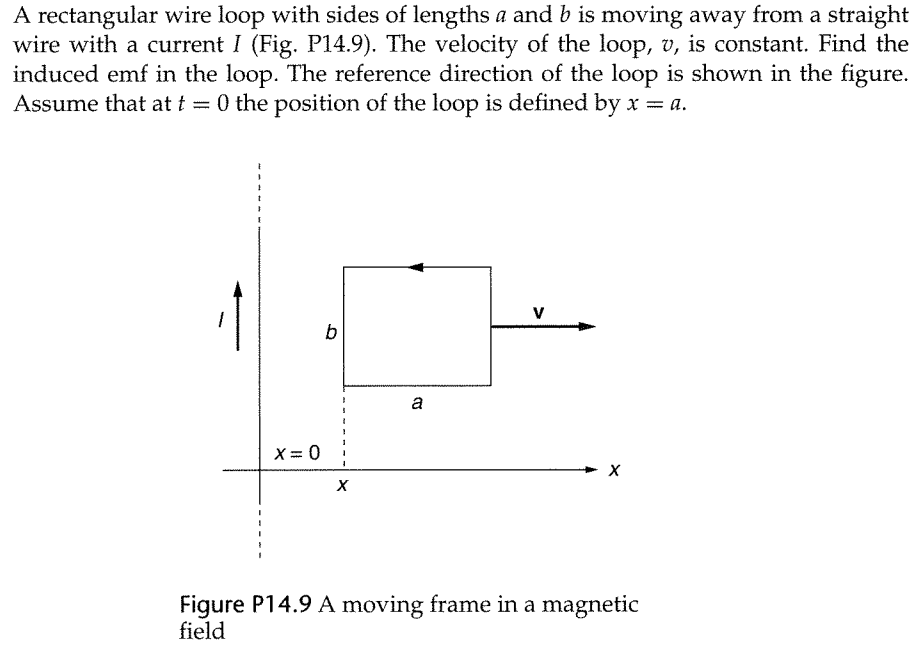
\includegraphics[width=14cm]{f1}
\end{center}
\end{figure}

We begin by finding the emf:

\[
  e = -\frac{d}{dt}\int_SB\cdot dS
\]
\[
  e = \frac{d}{dt}b\int_{x=vt}^{x=a+vt}\frac{\mu_0I}{2\pi x}\cdot dx
\]
\[
  e = \frac{d}{dt}\frac{\mu_0Ib}{2\pi}(\ln(a+vt)-\ln(vt))
\]
\[
  e = \frac{\mu_0Ib}{2\pi}(\frac{v}{a+vt} - \frac{1}{t})
\]
This should be positive since the induced current will try and oppose the magnetic field provided.
Since $B$ field provided goes into the page, the induced emf will be counterclockwise to create a
$B$ field out of the page.  Since there is a little arrow in the picture, that signifies the direction
of the surface vector (or so I pressumed).

\newpage
2) \textbf{15.8:}
\begin{figure}[H]
\begin{center}
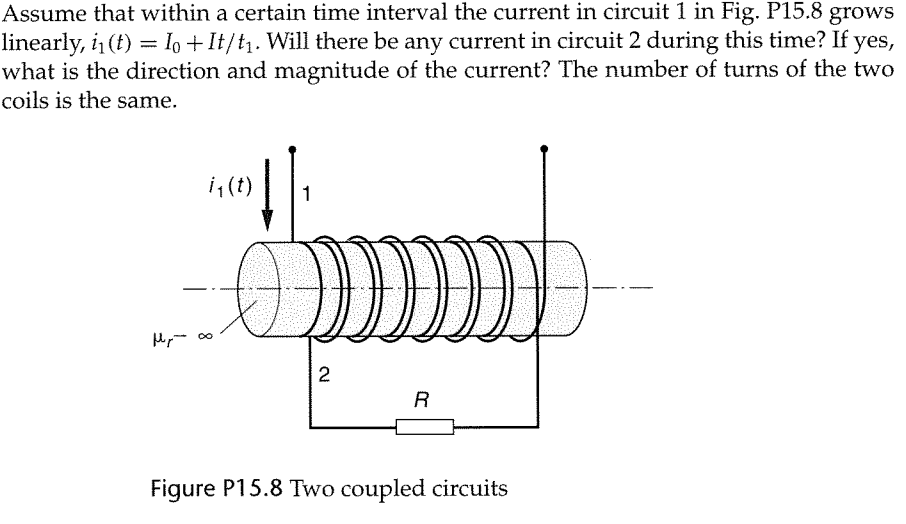
\includegraphics[width=14cm]{f2}
\end{center}
\end{figure}
There will be a current in circuit 2.  Since the magnetic field is identical within the two coils, the
induced emf in the second wire will be such as to generate an identical current.  The direction will be
as to oppose the induced field.  If we say that our current moves from left to right of the resistor then
the current will be:
\[
  i_2(t) = -i_1(t)
\]

\newpage
3) \textbf{15.12:}
\begin{figure}[H]
\begin{center}
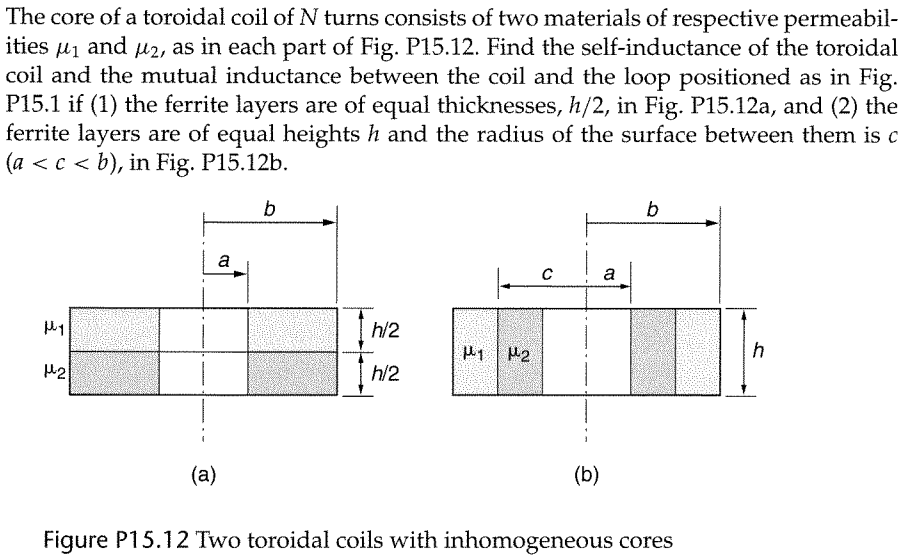
\includegraphics[width=14cm]{f3a}
\end{center}
\end{figure}
\begin{figure}[H]
\begin{center}
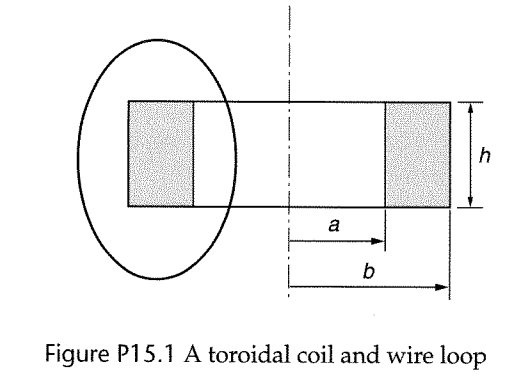
\includegraphics[width=7cm]{f3b}
\end{center}
\end{figure}

(a) The flux can be found:
\[
  d\Phi_{21}(r) = B(r)dS = \frac{\mu_1NI_2}{2\pi r} h_1+ \frac{\mu_2NI_2}{2\pi r} h_2dr
\]
\[
  \Phi_{21} = (\frac{\mu_1NI_2h_1}{2\pi} + \frac{\mu_2NI_2h_2}{2\pi})\int_a^b\frac{dr}{r} = (\frac{\mu_1NI_2h_1}{2\pi}+\frac{\mu_1NI_2h_1}{2\pi})\ln\frac{b}{a}
\]
Meaning that the mutual inductance is:
\[
  L_{12} = L_{21} = (\frac{\mu_1Nh_1}{2\pi}+\frac{\mu_2Nh_2}{2\pi})\ln\frac{b}{a}
\]
We have the flux though a cross section of the torus, this means we can easiliy find the self-inductance (since
the flux exists though $N$ turns of the wire, we find:)
\[
  L = \frac{(\mu_1+\mu_2)N^2h}{2\pi}\ln{\frac{b}{a}}
\]

(b) For this problem we need to use a different integral:
\[
  \Phi_{21} = \frac{NIh}{2\pi}(\int_a^c\frac{\mu_2dr}{r}+\int_c^b\frac{\mu_1dr}{r}) = \frac{NIh}{2\pi}(\mu_2\ln\frac{c}{a}+\mu_1\ln\frac{b}{c})
\]
The mutual inductance:
\[
  L_{12}=L_{21}=\frac{Nh}{2\pi}(\mu_2\ln\frac{c}{a}+\mu_1\ln\frac{b}{c})
\]
The self inductance is similarily:
\[
  L=\frac{N^2h}{2\pi}(\mu_2\ln\frac{c}{a}+\mu_1\ln\frac{b}{c})
\]

4) \textbf{15.17:}
\begin{figure}[H]
\begin{center}
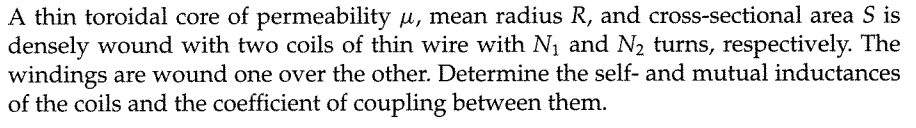
\includegraphics[width=14cm]{f4}
\end{center}
\end{figure}
Just like in the last problem, we know the self inductances to be:
\[
  L_1=\frac{\mu N_1^2S}{2\pi R} \text{ and } L_2=\frac{\mu N_2^2S}{2\pi R}
\]
The mutual inductance is given on page 268 of the textbook:
\[
  L_{12}=L_{21}=\frac{\mu N_1N_2h}{2\pi R}
\]
Interestingly, $\sqrt{L_1\times L_2} = L_{12}$ Which tells us that $k=1$.

\newpage
5) \textbf{16.4:}
\begin{figure}[H]
\begin{center}
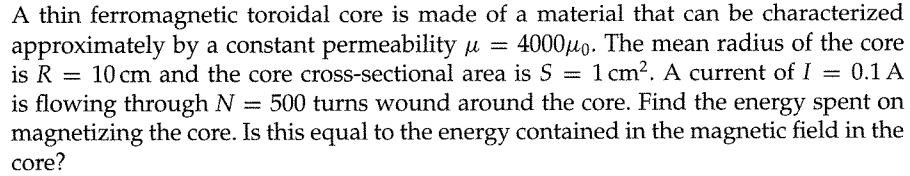
\includegraphics[width=14cm]{f5}
\end{center}
\end{figure}
We know that the inductance of a torroidal core is:
\[
  L=\frac{\mu N^2 S}{2\pi R}
\]
The magnetic energy in the coil is therefor:
\[
  W_m=\frac{1}{2}LI^2=\frac{I^2N^2\mu S}{4\pi R} = 1mJ
\]
The energy it takes to magnitize this device is equal to the amount of energy in theorem
magnetic field, due to conservation of energy.  This is also $1mJ$.

6) \textbf{16.17:}
\begin{figure}[H]
\begin{center}
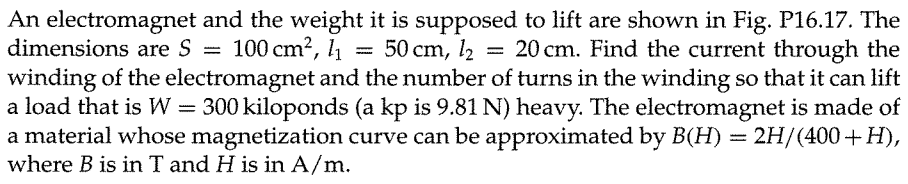
\includegraphics[width=14cm]{f6a}
\end{center}
\end{figure}
\begin{figure}[H]
\begin{center}
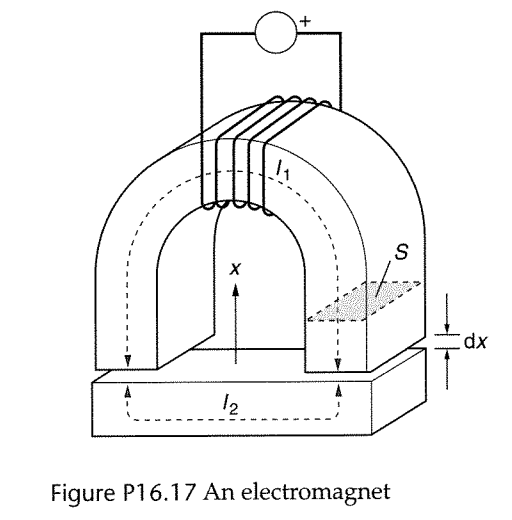
\includegraphics[width=5cm]{f6b}
\end{center}
\end{figure}
\newpage
The force is equal to:
\[
  F=\frac{1}{2}\frac{B^2}{\mu}2S
\]
We need
\[
  300*9.81=\frac{2H^2}{\mu(400+H)}2(1)
\]
In order to lift this we need an H field of $0.6086 H$.  To generate A field
of this magnetude we will need a current of:
\[
  0.61=\frac{I}{2A} \Rightarrow I = 0.61*2S = 0.0122 A
\]

7) \textbf{17.1:}
\begin{figure}[H]
\begin{center}
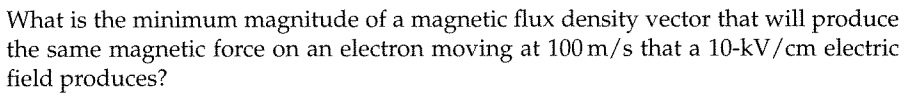
\includegraphics[width=14cm]{f7}
\end{center}
\end{figure}
The force from this E-field is:
\[
  F = QE = -0.2pN
\]
This mus be equal to:
\[
  -0.2pN = Qv \times B
\]
If the B field is in the same direction
\[
  B = \frac{-0.2p}{Qv} = 10 kT
\]
\newpage
d8) \textbf{18.1:}
\begin{figure}[H]
\begin{center}
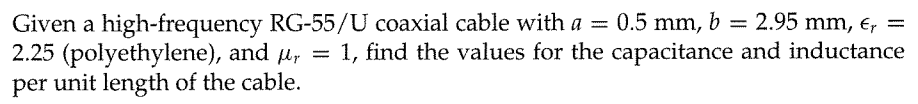
\includegraphics[width=14cm]{f8}
\end{center}
\end{figure}
These are from the textbook:
\[
  C' = \frac{2\pi\epsilon}{\ln(b/a)}
\]
\[
  L' = \frac{\mu_r}{2\pi}\ln\frac{b}{a}
\]

9) \textbf{18.5:}
\begin{figure}[H]
\begin{center}
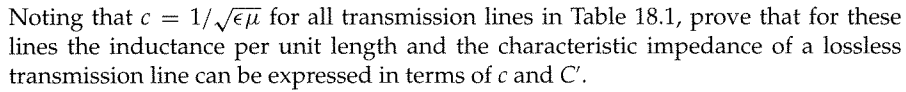
\includegraphics[width=14cm]{f9}
\end{center}
\end{figure}
Some alegebra and we can see:
\[
  L'=\frac{1}{c^2C'} \text{ and } Z_0 = \frac{1}{cC'}
\]
For all of these.

\end{document}
